\chapter{Validation Exercises for Lava Flow Algorithms}\label{apdx_lava}

\renewcommand*{\FigPath}{figures/chapter-molasses}
%%%%%%%%%%%%%%%%%%%%%%%%%%%%%%%%%%%%%%%%%%%%%%%%%
%MOLASSES%%%%%%%%%%%%%%%%%%%%%%%%%%%%%%%%%%%%%%%%
%%%%%%%%%%%%%%%%%%%%%%%%%%%%%%%%%%%%%%%%%%%%%%%%%
%%%%%%%%%%%%%%%%%%%%%%%%%%%%%%%%%%%%%%%%%%%%%%%%%
%%%%%%%%%%%%%%%%%%%%%%%%%%%%%%%%%%%%%%%%%%%%%%%%%

\section{A modular cellular automata framework for lava flow simulators}\label{sec:MOLASSES}

CA in lava flows has historically been defined as a 2-dimensional space, which is divided into equal-area grid cells, such as those found in a common digital elevation model (DEM). Within the location of each cell is defined an ``elementary automaton'' (\textit{ea}) that has a set of properties, is governed by a set of global rules, and has a set list of neighboring automata. While the behavior rules that each \textit{ea} follow is identical to those of all other automata, its behavior is only dictated by local phenomena. Specifically, the amount of lava that flows in or out of an \textit{ea} will depend on properties such as lava thickness and elevation within it and its neighbors. Because grid cells and \textit{ea} are fundamentally inseperable in this application, I will refer to \textit{ea} as cells.

The set of cellular automata is defined as
	\begin{equation}
		\mathbf{A} = \mathrm{\{E^2, V, S, X, \sigma, \gamma\}}
	\end{equation}
	where E$^2$ is the set of point locations of cells in \textbf{A}, V$\subset$E$^2$ is the set of vent or source locations, S is the set of substates within each cell, and X is the local neighborhood that each cell can directly influence \citep{barca1994cellular}. $\sigma$ and $\gamma$ represent the transition functions and source functions within \textbf{A}. 
	
	Practically, E$^2$ is a set of coordinate pairs denoting row and column addresses of cells in a larger grid. S($i$,$j$), which represents the set of substates for the cell at row $i$, column $j$, includes S$_e$, the underlying elevation of an automaton; S$_h$, the thickness of lava within the cell; and S$_{h0}$, the critical thickness, above which lava will spread from a cell. Some algorithms include S$_T$, or the cell temperature in this set. X, in a four-connected neighborhood scheme, is given as \{(0,1), (0,-1), (1,0), (-1,0)\}, where (0,0) is the location of a cell under evaluation. $\sigma$ is the change of substates in S for each cell from timestep $t$ to $t+1$, or S$^{t}\rightarrow$S$^{t+1}$. $\gamma$ specifies the lava emitted at locations within V. The implementation of these sets within the CA structure \textbf{A} is described in detail below.
	
	\subsection{MOLASSES algorithm outline}
		MOLASSES is a Cellular Automata code developed in the C programming language based on the CA algorithm ``LavaPL'' of \citet{connor2012probabilistic}. The major change between LavaPL and MOLASSES is that MOLASSES is constructed with nine modules that each have a specific task, either carrying out the CA simulation, reading model input, or writing model output (Figure \ref{fig_flowchart}). The nine modules were designed to replicated major functions in LavaPL and are:
		\begin{enumerate}
			\item{\textbf{DRIVER}} Calls modules in sequence to execute the flow algorithm.
			\item{\textbf{INITIALIZE}} Reads a user-provided configuration file to define model parameters.
			\item{\textbf{DEM\_LOADER}} Imports a raster file to define the elevation model.
			\item{\textbf{INITFLOW}} Uses model parameters to define data arrays.
			\item{\textbf{PULSE}} Incrementally adds lava to source locations.
			\item{\textbf{DISTRIBUTE}} Determines whether to spread and how to spread lava between cells.
			\item{\textbf{NEIGHBOR\_ID}} Identifies the cell neighborhood.
			\item{\textbf{ACTIVATE}} Adds newly inundated cells to the list of active cells.
			\item{\textbf{OUTPUT}} Writes model results to a file using user-specified formats.
		\end{enumerate}
		
		\begin{figure}[!h]
			\centering
			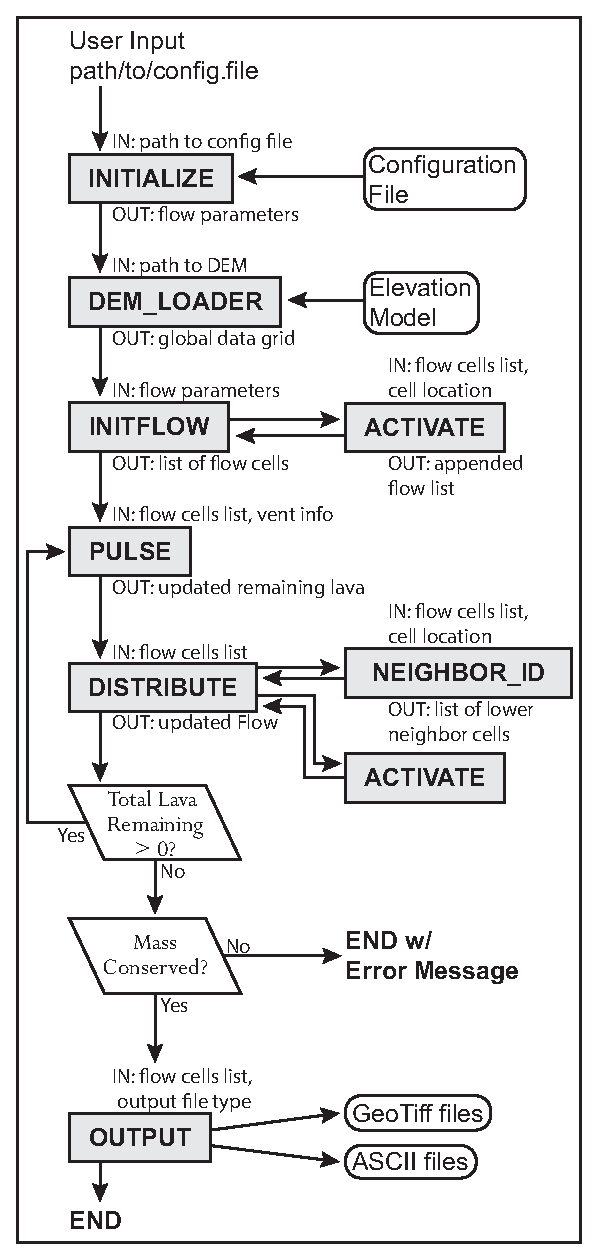
\includegraphics[width=0.3\linewidth]{\FigPath/Flow_Chart}
			\caption[A flow chart of MOLASSES carried out within the \textbf{DRIVER} module]{A flow chart of MOLASSES carried out within the \textbf{DRIVER} module. Gray boxes denote various modules, with major inputs and outputs given above and below. Parallelograms are checks performed within DRIVER itself. Rounded boxes represent external input and output files.}
			\label{fig_flowchart}
		\end{figure}
		
		
		Like LavaPL, model parameters are specified by a user through a text configuration file, which must include 1) a digital elevation model (DEM), 2) a residual lava flow thickness, 3) at least one vent location, 4) the total volume and ``pulse volume'' of this vent, and 5) an output file path. The lava flow thickness defines the CA value of S$_{h0}$, where cells with flow thicknesses S$_h>$S$_{h0}$ will spread all lava to their neighboring cells, while cells with less lava will retain their lava. The ``pulse volume'' defines $\gamma$ and the amount of lava to emit at the source location at each time step. The total volume constrains $\gamma$ as lava will not be introduced to the source location after the total volume has been delivered. Modules within MOLASSES that further execute the CA simulation are detailed below.
		
	\subsection{Cells in E$^2$}
		%DEM_LOADER
		%INITFLOW
		%ACTIVATE
		Information for cells in the grid defined by E$^2$ is stored in two ways, for code efficiency. First, some information of the CA structure \textbf{A} is stored in a Global Data Grid. This grid stores information known at the beginning of the simulation, such as the user supplied residual flow thickness and the elevation. Grid dimensions are set in the \textbf{DEM\_LOADER} module to be identical to the user-specified raster DEM. This module then imports the elevation of each raster pixel into the corresponding grid cell location. After this operation, the residual flow thickness is also stored in the grid.

		The second information storage method is a list defined in the \textbf{INITFLOW} module. The ``Active List'' is declared with a length that corresponds to the theoretical maximum number of cells that can be inundated by lava. This list contains data that is updated during the simulation, including lava thicknesses, $S_h$, within cells. As cells are determined within the simulation to be inundated with lava for the first time, their row and column addresses, as well as their lava thicknesses are appended to the Active List with the module \textbf{ACTIVATE}.
		
	\subsection{Source locations, V, and the source function, $\gamma$}
		%INITFLOW
		%PULSE
		Initially in the Active List, \textbf{INITFLOW} only declares source location(s) as the first few elements of the list. These source locations are flagged in the list to be identified as source locations by other modules.

		The \textbf{PULSE} module carries out the source function, $\gamma$. In this module, a separate array stores each source vent's volume parameters. The pulse volume is added to the quantity of lava in the source cell and is subtracted from the remaining volume. The remaining volume is initially set as the total volume given in the configuration file, so PULSE continues to add lava to the source locations at each time step until remaining volume is 0.
		
	\subsection{Substates, S, and the transition function, $\sigma$}
		%INITFLOW
		%DISTRIBUTE
		Substates which cannot change, such as the cell elevation S$_e$ and the residual flow thickness S$_{h0}$, are stored within the Global Data Grid. Substates which do change, primarily flow thickness, S$_h$, are stored in the Active List and are allowed to change from timestep to timestep. These values are initialized in \textbf{INITFLOW} where thicknesses are set to 0.
		
		The transition function, $\sigma$, is defined in the \textbf{DISTRIBUTE} module. Cells in this module are evaluated in order of their inundation (i.e. vents are evaluated first and distal cells are evaluated last). The incoming and outgoing quantity of lava from each cell is stored in the Active List. Generally, if a cell has a flow thicknesses S$_h>$S$_{h0}$, it will spread the lava above S$_{h0}$ to any neighbors lower in elevation than itself. When all inundated cells have been evaluated, the incoming and outgoing quantities of lava of each cell are applied to the cells. This flow transition represents a timestep as all cells are updated at once.
		
		Multiple possible transition functions can effectively spread lava from and to cells in a manner that might replicate lava in real life. Identifying transition functions that spread lava in a realistic way is the purpose of the validation tests described in Section \ref{sec_validationb}. In this project three main variations are combined and tested which vary 1) how local slope affects spreading, 2) the neighborhood size, and 3) if any neighbors are eliminated from the neighborhood based on their relationship to the cell.
		\begin{figure}[!h]
			\centering
			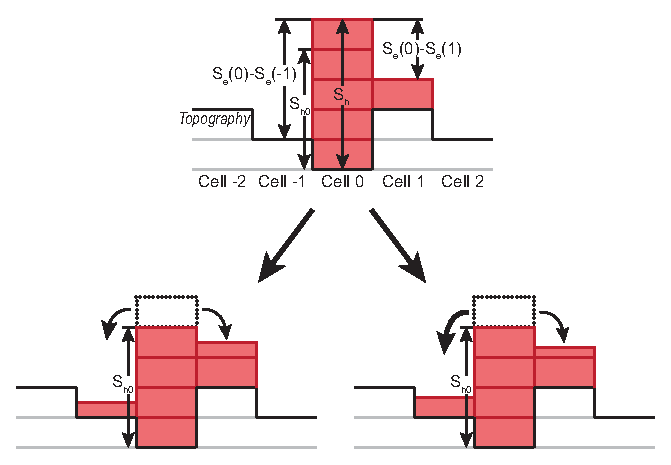
\includegraphics[width=0.5\linewidth]{\FigPath/slope-proportional-example}
			\caption[A 2-D example of two transition functions with different slope treatments]{A 2-D example of two transition functions with different slope treatments. At timestep $t$ (top), Two cells are inundated with lava. The central cell (Cell 0) has 1 block of lava higher than the residual thickness, S$_{h0}$. In a slope-proportional sharing scheme, timestep $t+1$ will follow the path to the right; because Cell -1 has twice the relief as Cell 1, it receives twice as much of the residual lava (2/3 blocks vs. 1/3 to the right). In an equal-sharing scheme, the left path will be followed, and half the block will be added to both neighbor cells.}
			\label{fig_BernieSanders}
		\end{figure}

		\paragraph{Local slope-based spreading} In the LavaPL algorithm given by \citet{connor2012probabilistic}, lava is apportioned from cells to their neighboring cells proportional to slope. To give a specific case, let a cell at location $c$ be the central cell, with a set of neighbor cells, X. The total relief between cell $c$ and its lower neighboring cells is
		\begin{equation}
			\text{TR}(c) = \sum^{n\in \text{X}}(\text{S}_h(c)+\text{S}_e(c))-(\text{S}_h(n)+\text{S}_e(n))
			\label{eq_TR}
		\end{equation}
		where $\text{S}_h$ is the height or thickness of the lava in a cell, $\text{S}_e$ is the underlying elevation of the cell, and $n$ is a neighbor in X. The total lava to spread away from the central cell is the difference between thickness of lava (S$_h$) at $c$ the residual thickness (S$_{h0}$), unless the lava thickness is lower than the residual thickness, giving
		\begin{equation}
			\text{Outbound}(c) =
			\begin{cases}
			\text{S}_h(c)-\text{S}_{h0}(c) & \quad \text{if } {S}_h(c)-\text{S}_{h0}(c) > 0\\
			0 & \quad \text{if } {S}_h(c)-\text{S}_{h0}(c) \le 0\\
			\end{cases}
			\label{eq_excess}
		\end{equation}
		
		In LavaPL, the excess flow, ``Outbound'', is delivered to neighbors $n$ based on the proportion of total relief, TR, found at each neighbor location (the right path of Figure \ref{fig_BernieSanders}). For each $n\in$X,
		\begin{equation}
			\text{Inbound}(n) = \text{Outbound}(c)\left(\frac{(\text{S}_h(c)+\text{S}_e(c))-(\text{S}_h(n)+\text{S}_e(n))}{\text{TR}}\right)
			\label{eq_propshare}
		\end{equation}
		This is the slope-proportional spreading equation. Another method would be ``slope-blind,'' and would spread lava to all lower neighbors equally following the equation
		\begin{equation}
			\text{Inbound}(n) = \left(\frac{\text{Outbound}(c)}{|\text{X}|}\right)
			\label{eq_equalshare}
		\end{equation}
		where $|\text{X}|$ is the size of the neighborhood, or the number of elements in the neighborhood. This is illustrated as the left path of Figure \ref{fig_BernieSanders}.
		
		\paragraph{Neighborhood size} The size of the neighborhood, X, in CA algorithms is commonly 4 or 8 in cardinal or ordinal directions. Here both have been implemented and both 4- and 8- connected neighborhoods are evaluated in validation exercises later. Neighborhood size is further described in the next section (\ref{sec_X}).

		\paragraph{Spreading inhibited by special relationships} Though the size of the neighborhood is set globally for all cells, neighbors are not guaranteed to receive lava from central cells. In all algorithms, for example, cells in the neighborhood that are higher than the central cell, including lava thicknesses, are excluded from the neighborhood set.
		
		\begin{figure}[!h]
			\centering
			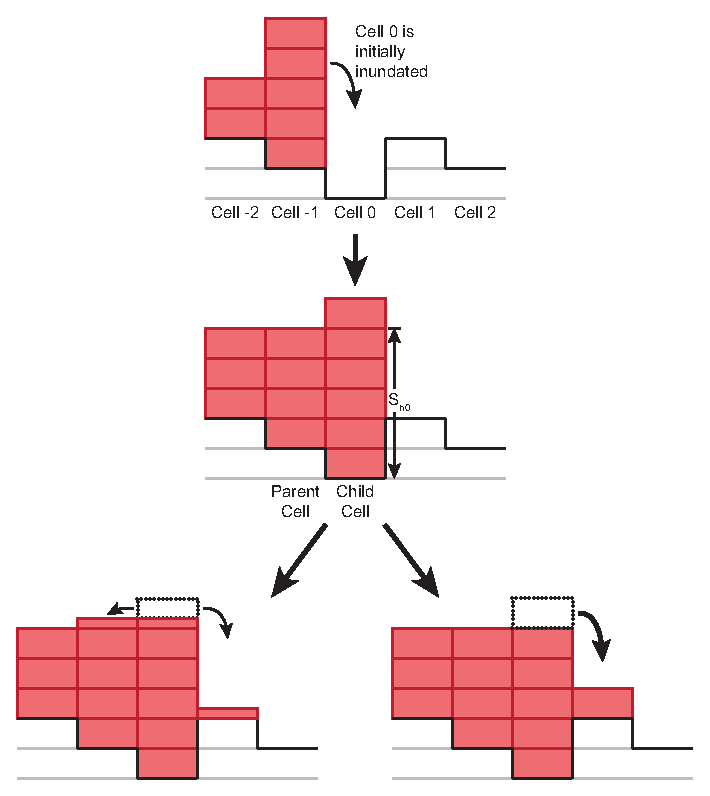
\includegraphics[width=0.5\linewidth]{\FigPath/parent-child-example}
			\caption[A 2-D example of different transition functions with different ``parentage'' rules]{A 2-D example of different transition functions with different ``parentage'' rules. In the first timestep (top), Cell -1 initially inundates Cell 0, creating the Parent-Child relationship shown in the next illustrated timestep (middle). If Parents cannot receive lava from Child cells, all residual lava in Cell 0 will flow to Cell 1, following the path to the right. If these relationships are ignored, as shown in the left path, Cell 0 will spread lava in both directions.}
			\label{fig_ParentTrap}
		\end{figure}
		
		Other neighbor elimination rules can also be implemented. One has been designed by \citet{connor2012probabilistic}, where the cell that initially gives lava to another cell is forever eliminated from the receiving cell's neighborhood. This is done by creating a ``parent-child'' relationship for each activated cell in the flow. Simply put, child cells cannot give lava to their parent cells (right path in Figure \ref{fig_ParentTrap}). This transition function rule is tested against no parentage rules in competing MOLASSES algorithms (left path in Figure \ref{fig_ParentTrap}).
		
	\subsection{Cell neighborhood, X}\label{sec_X}
	
	\begin{figure}[!h]
		\centering
		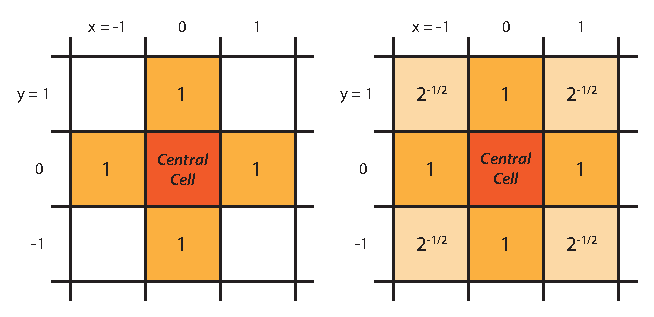
\includegraphics[width=0.5\linewidth]{\FigPath/neighborhoods}
		\caption[Cellular Automata neighborhoods]{Cellular Automata neighborhoods. To the left, in a 4-connected neighborhood, a central cell may influence or be influenced by cells in cardinal directions. To the right, in an 8-connected neighborhood, the zone of influence is expanded to include ordinal directions. Numbers in each cell are relative weights (determined by distance from the central cell), so diagonal neighbors are weighted less than orthogonal cells.}
		\label{fig_MrRogers}
	\end{figure}
	
		%NEIGHBOR_ID
		The final set in the CA is the cell neighborhood X and is defined by the \textbf{NEIGHBOR\_ID} module. This neighborhood is usually either 4-connected (von Neumann neighborhood) or 8-connected (Moore neighborhood) as illustrated in Figure \ref{fig_MrRogers}. Four-connected neighborhoods are defined as the row, column coordinates \{(0,1), (0,-1), (1,0), (-1,0)\}, where (0,0) is the location of a cell under evaluation, while the set elements might correspond to North, South, East, and West. Eight-connected neighbors include the ordinal directions, Northeast, Southeast, Northwest, and Southwest: \{(0,1), (0,-1), (1,0), (-1,0), (1,1), (-1,-1), (1,-1), (-1,-1)\}.
		
		NEIGHBOR\_ID is implemented within the DISTRIBUTE module to evaluate cells within X, and determine whether they are lower in elevation (including their lava) than the central cell. If one is lower, NEIGHBOR\_ID returns their relief, or the difference in elevation between the cell and the central cell, to the DISTRIBUTE module. Depending on whether parent-child relationships are recorded or ignored in the transition function, NEIGHBOR\_ID can follow one of two algorithms outlined in Table \ref{tab_neighalg}.
	\begin{table}[h]
		\centering
		\caption{NEIGHBOR\_ID Module Algorithms}
		\begin{tabular}{l}
			\toprule
			\textbf{4-connected NEIGHBOR\_ID}\\
			\textbf{module}\\
			\midrule
			X = \{(0,1), (0,-1), (1,0), (-1,0)\}\\\\
			X' = \{\}\\
			$c$ = (0,0)\qquad (central cell location)\\
			\textbf{For} $n\in$ X\\
			~~\textbf{If}~$(\text{S}_h(c)+\text{S}_e(c))-(\text{S}_h(n)+\text{S}_e(n)) > 0$\\
			~~~~\textbf{Append}~$n$ to X'\\\\
			\textbf{Return}~X'\\
			\bottomrule
		\end{tabular}
		\begin{tabular}{l}
			\toprule
			\textbf{8-connected NEIGHBOR\_ID}\\
			\textbf{with Parent-Child Relationships}\\
			\midrule
			X = \{(0,1), (0,-1), (1,0), (-1,0), \\
			\qquad~(1,1), (-1,-1), (1,-1), (-1,-1)\}\\
			X' = \{\}\\
			$c$ = (0,0)\qquad (central cell location)\\
			\textbf{For} $n\in$ X\\
			~~\textbf{If}~$(\text{S}_h(c)+\text{S}_e(c))-(\text{S}_h(n)+\text{S}_e(n)) > 0$\\
			~~~~\textbf{If} $n$ is \textbf{not} Parent of $c$\\
			~~~~~~\textbf{Append}~$n$ to X'\\
			\textbf{Return}~X'\\
			\bottomrule
		\end{tabular}
		\label{tab_neighalg}
	\end{table}
			
%%%%%%%%%%%%%%%%%%%%%%%%%%%%%%%%%%%%%%%%%%%%%%%%%%
%HIERARCHY
%%%%%%%%%%%%%%%%%%%%%%%%%%%%%%%%%%%%%%%%%%%%%%%%%%

	\section{Validation hierarchy}\label{sec_validationb}
	
	The validation strategy implemented in this paper follows the advice of \citet{bayarri2007framework} for validating computer models, namely ``1) defining the problem; 2) establishing evaluation criteria; 3) designing experiments; 4) approximating computer model output; 5) analyzing the combination of field and computer run data.'' The sixth step in their validation process, feeding results back to revise models, has been done informally to determine how to alter spreading algorithms in the future. Each level below presents a problem for a lava spreading algorithm to complete. These fundamental problems (e.g. replicating a Bingham flow) are evaluated using simple tests that demonstrate the problem. The relevant model output for each of these tests is a list of locations (i.e. a list of x and y coordinates) that have been inundated by lava. After verification (Level 0), the first validation level tests model results with other model results; the second level tests model output against expected analytical solutions; and the third level tests model output from field data. 
	
	Multiple flow algorithms can pass all of these tests, illustrating that they are valid under certain conditions and can be relied on. Choosing between algorithms which have been validated is based on the needs of the user, but algorithms that do not perform well in these validation tests might not be reliable for other applications.

		\begin{table}[h]
		\centering
		\caption{Transition Algorithm Codes and Descriptions}
		\begin{tabular}{l c p{5cm} p{5cm}}
			\toprule
			Transition&Neighborhood&Parent-Child&Slope-proportional\\
			Function&&Relationships Preserved?&Sharing?\\
			\midrule
			\textbf{4/P/S} &4-directions & Yes, ``parents'' do not accept lava from ``children.'' & Yes, lower cells receive lava based on relative relief.\\
			\textbf{8/P/S} &8-directions & Yes & Yes\\
			\textbf{4/N/S} &4-directions & No, ``parents'' are not defined. & Yes\\
			\textbf{8/N/S} &8-directions & No  & Yes\\
			\textbf{4/P/E} &4-directions & Yes & No, all lower cells receive equal quantities of lava.\\
			\textbf{8/P/E} &8-directions & Yes & No\\
			\textbf{4/N/E} &4-directions & No  & No\\
			\textbf{8/N/E} &8-directions & No  & No\\
			
			\bottomrule
		\end{tabular}
		\label{tab_algorithmcodes}
		\end{table}

\paragraph{Test algorithms} Combining three variations of the Transition Function described in Section \ref{sec:MOLASSES}, I have created eight MOLASSES lava flow algorithms. Each variation has been made by modifying one module in the MOLASSES framework: The neighborhood is changed between 4- and 8- directions using the NEIGHBOR\_ID module, classifying one cell as a ``parent'' cell when a location is initially inundated is within the ACTIVATE module, and dividing lava amongst neighboring cells proportional to slope or equally is carried out in the DISTRIBUTE module. These eight algorithms will be referred to using three character codes, listed in Table \ref{tab_algorithmcodes}. For the algorithm used by LavaPL in \citet{connor2012probabilistic}, the code would therefore be 4/P/S, as it spreads lava in 4-directions from a central cell, all inundated cells have designated parents to whom they cannot spread lava, and the quantity of lava to spread from a central cell is higher for lower neighboring cells.

	\subsection{Level 0: Conservation of mass}
			Before the results of a lava flow simulation can be validated, it must be verified to at least prove that conservation of mass is preserved. A lava flow simulation will therefore not be tested against the following tests until this conservation of mass requirement is shown to be fulfilled.
			
			In MOLASSES, the code is verified within the DRIVER module, which manages each subordinate module. The erupted volume, $V_{in}$, is given as the total eruption volume specified by the user in the configuration file. If multiple source locations are given in this file, $V_{in}$ is the sum of total eruption volumes. $V_{in}$ is compared at the end of the module to the total volume of the flow, or $V_{out}$. The volume $V_{out}$ is calculated by summing the volume in all inundated grid cells. MOLASSES reports success if $V_{in}-V_{out} \le 10^{-8}$~m$^3$, which is the precision of a 64-bit double. If this test fails, MOLASSES reports failure and the excess volume found in the flow (Table \ref{tab_masscons}).
	
			\begin{table}[h]
				\centering
				\caption{MOLASSES Conservation of Mass Test}
				\begin{tabular}{l}
					\toprule
					\textbf{If}~$|V_{in}-V_{out}| \le 10^{-8}$\\
					~~\textbf{Print}~\verb|SUCCESS: MASS CONSERVED|\\
					\textbf{Else}\\
					~~$excess = V_{out}-V_{in}$\\
					~~\textbf{Print}~\verb|ERROR: MASS NOT CONSERVED! Excess: |$excess$ \verb|m^3|\\
					\bottomrule
				\end{tabular}
				\label{tab_masscons}
			\end{table}

	\subsection{Level 1: Repeatability given meaningless parameter variation}
		Once the code has been verified to conserve mass, the flow can be validated. This first validation level tests that lava flow simulations are repeatable, regardless of changes in parameter space that should have no effect on the flow. Parameters that ideally should not effect lava flows include slope direction and elevation model resolution. For instance, a slope to the west and an identically dipping slope to the east should produce lava flows of equal length and shape (given identical flow attributes).
		
		\citet{miyamoto1997simulating} performed a simple validation test on two CA-like flow simulators \citep{ishihara1990numerical,miyamoto1997simulating} where a sloped DEM was rotated 45 degrees from ``south'' to ``southeast''. This test was performed to demonstrate that the flow models had the same run-out length regardless of the arbitrary slope direction. Here, the DEM rotation scheme by \citet{miyamoto1997simulating} is adopted and expanded, so that a DEM of a simple slope is rotated 19 times at increments of 5$^{\circ}$. Flows are simulated on each of these slopes and the locations of inundated cells are output from the model.
		
		Three characteristics of the simulated flows are determined for each slope direction: flow length, orientation, and aspect ratio. Flow length is defined as the distance between the vent and the furthest inundated point from the vent. Flow orientation is defined as the direction that furthest point lies, with respect to North. Flow aspect ratio is the ratio of maximum flow width to flow length. Perfect success for this exercise is when simulated flows, regardless of slope direction, 1) do not change in length, 2) have an orientation identical to the slope direction, and 3) do not change in aspect ratio. Failure is more subjective, but I will define failure as 1) more than 10\% variation in flow length depending on slope direction, 2) more than 5$^{\circ}$ offset between the slope and the flow orientation on average, or 3) more than 15\% variation in flow aspect ratio.
		
		\begin{figure}[h!]
			\centering
			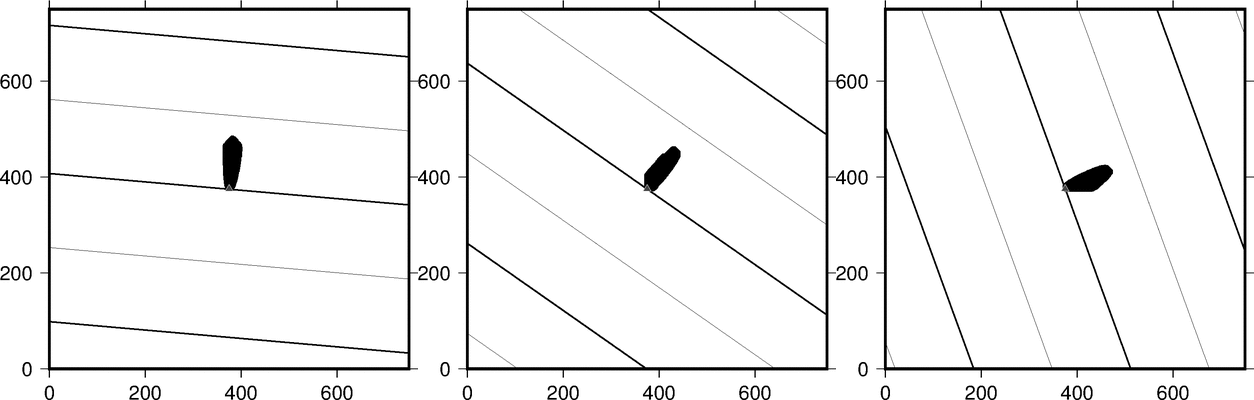
\includegraphics[width=\linewidth]{\FigPath/lava_C_4N_slope}
			\caption[Rotating slope test for algorithm \textbf{4/P/S} (LavaPL)]{Rotating slope test for algorithm \textbf{4/P/S} (LavaPL). Slope dip is 18$^{\circ}$, with dip-directions 0N, 30N, and 80N from left to right. The flow length and aspect ratio are similar and the flow direction is in the slope direction, so it passes Level 1 criteria.}
			\label{fig:slope}
		\end{figure}
		
		\subsubsection{Exercise parameters} The underlying DEM for this exercise has a simple 18$^{\circ}$ slope, dipping to the North. The DEM has a spatial resolution of 1~m. The source cell is placed at the center of the DEM, is given a total volume of 1000~m$^3$, and is given a pulse volume of 1~m$^3$. When the simulation is finished, model output is used to determing the three flow characteristics used in this test (length, orientation, and aspect ratio). The DEM is rotated 5$^{\circ}$ clockwise and the process is repeated 19 times until the flow is simulated on an East-facing slope.
		
		
		
		\subsubsection{Results}

		For all eight flow algorithms, flow length, aspect ratio, and orientation were calculated 19 times, corresponding to the 19 dip directions sampled between 0$^{\circ}$N and 90$^{\circ}$N. Variance for length and aspect ratio were calculated as the ratio of their standard deviations to their means. For instance, if mean runout length for the 18 flows is 100~m and the standard deviation of the 18 lengths is 2~m, the runout length variance is 2\%. The mean direction error is also calculated for the set of flows from each algorithm. These results are reported in Table \ref{tab_rotresults}.

			\begin{table}[h]
				\centering
				\caption{DEM Rotation Results}
				\begin{tabular}{l c c c}
					\toprule
					Transition&Run-out&Aspect Ratio&Mean Direction\\
					Function&Variance&Variance&Error\\
					\midrule
					4/P/S &2.7\%&6.7\%&1.2$^{\circ}$\\
					8/P/S &4.4&12.2&0.9\\
					4/N/S &9.6&19.7&1.3\\
					8/N/S &3.9&7.5&0.6\\
					4/P/E &21.6&38.6&14.2\\
					8/P/E &7.2&13.8&5.4\\
					4/N/E &21.6&38.7&14.1\\
					8/N/E &7.2&13.8&5.5\\
					\bottomrule
				\end{tabular}
				\label{tab_rotresults}
			\end{table}

			While with an ideal spreading algorithm, variances and direction error would be 0 under a rotating slope, every spreading algorithm tested performed differently as DEM direction changed. Following from the above pass-fail standards, five of the eight algorithms can be rejected. Algorithms 4/P/E and 4/N/E have high run-out length variance. Algorithms 4/N/S, 4/P/E and 4/N/E have large aspect-ratio variance. Algorithms 4/P/E, 8/P/E, 4/N/E, and 8/N/E all systematically deviate from running downslope by $>5^{\circ}$ on average. This implies that algorithms which share lavas equally from central cells to all lower neighboring cells perform worse than algorithms which share lavas proportional to slope.
			
			For the eight different transition functions tested, runout length varied between 60-160~m. The flow algorithm with the least flow length variance was the 4-connected, parent-child, slope-proportional strategy implemented in LavaPL. Algorithms 4/P/S (LavaPL), 8/P/S, and 8/N/S cannot be rejected because of any of the three standards set in this exercise.

	\subsection{Level 2: Replication of flow morphologies on simple physical surfaces}
	
	The second validation level is the first step in validating lava flow algorithms against realistic flow expectations. Instead of parameter space being arbitrarily defined, which was the case in Level 1, the defined parameter space informs tests at this level as to what the model output should be. As lava flows on a large scale are well described as Bingham fluids, simulations can be tested against analytical solutions or experimental observations of these fluids in simple conditions. For instance, a lava flow on a perfectly flat surface might be expected to create a circular areal extent \citep{griffiths2000dynamics}.
	
			Here I measure flow algorithm performance on a flat surface from a single vent source location. To measure the extent to which the simulated flow replicates a circle, the inundated area is compared to the area of a circle which circumscribes the flow exactly. This can be described as
			\begin{equation}
				Fit = \frac{A_{flow}}{\pi d_{max}^2}
			\end{equation}
			where $d_{max}$ is the farthest extent of the simulated flow from the vent. A perfect match to a circle would result in a $Fit=1$. With the same maximum distance from the vent (i.e. the distance from the center to a vertex) a perfect square would cover 64\% of the area of a circle, ergo $Fit=0.64$. An octagon would have a fit of 0.90. We consider a model to successfully pass this test if it produces a flow of $Fit>0.90$, or if the flow approximates a circle better than an octagon. The model unambiguously fails this test if if produces a flow of $Fit<0.64$, where a square better describes a circle than a flow generated from the model. These thresholds are listed in Table \ref{tab_circtest}.

			\begin{table}[h]
				\centering
				\caption{Circular Flow Test Thresholds}
				\begin{tabular}{l l}
					\toprule
					Fit = 1.0 & Best Possible Score; perfectly circular.\\
					Fit $>$ 0.90 & Success; better than an octagon. \\
					Fit $<$ 0.64 & Failure; worse than a square.\\
					\bottomrule
				\end{tabular}
				\label{tab_circtest}
			\end{table}
		
		\begin{figure}[!h]
		\centering
		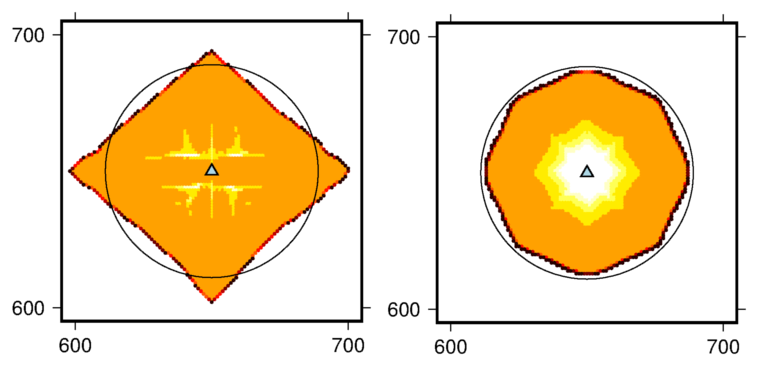
\includegraphics[width=\linewidth]{\FigPath/pancake}
		\caption[Fitness scores of different shaped flows on a flat surface]{Fitness scores of different shaped flows on a flat surface. From left to right: A circle has a perfect fit score of 1.00; an octagon has 0.90 times the area of a circumscribing circle; a square has a score of 0.64; Two flat surface tests for slope proportional spreading algorithms with parent rules. The flow second to the right is 4-connected (4/P/S) and has a score of 0.55, while the rightmost flow is 8-connected (8/P/S) with a score of 0.95. While the 4/P/S flow scores worse than a square, its 8-connected version passes the test as it scores better than an octagon.}
		\label{fig_pancake}
	\end{figure}
	
		\subsubsection{Exercise parameters} The DEM used in this exercise is a horizontal plane (all grid locations have the same elevation) with a spatial resolution of 1~m. A single vent is located at the DEM center with a total volume of 1000~m$^3$, and a pulse volume of 1~m$^3$. When the simulation is finished, model output is used to find the inundated cell farthest from the vent ($d_{max}$). The total inundated area is divided by the area of a circle with radius $d_{max}$ to provide the Fit score.
		
		\subsubsection{Results}

		Five of the eight algorithms unambiguously passed the test of performing better than an octagon (Table \ref{tab_circresults}). In this test 8-connected algorithms outperformed 4-connected algorithms. Four algorithms unambiguously passed this test: 8/P/S, 8/N/S, 4/N/E, and 8/N/E.
		
		\begin{table}[h]
			\centering
			\caption{Bingham Circle Results}\\
			\begin{tabular}{l c l}
				\toprule
				Algorithm&Circularity&\\
				\midrule
				4/P/S & 0.55 & Worse than a square.\\
				8/P/S & 0.95 & Better than an octagon.\\
				4/N/S & 0.55 & Worse than a square.\\
				8/N/S & 0.98 & Better than an octagon.\\
				4/P/E & 0.77 & Between a square and an octagon.\\
				8/P/E & 0.80 & Between a square and an octagon.\\
				4/N/E & 1.00 & Perfectly circular.\\
				8/N/E & 0.99 & Better than an octagon.\\
				\bottomrule
			\end{tabular}
			\label{tab_circresults}
		\end{table}
		
	\subsection{Level 3: Replication of real lava flows over complex topography}\label{sec_tolb_bench}
		The recent availability of global or near-global topographic datasets, such as SRTM or ASTER GDEM has enabled the direct observation of the underlying surface of even more recent lava flows. Flow algorithms can be validated against recent lava flows by simulating lava over these surfaces with parameters defined by the new lava flows. The 2012-3 Tolbachik lava flows will be used as a validation exercise for the eight flow algorithms. As discussed above (Section \ref{sec_tolb_back}), the earliest lavas flowed from a fissure to the west. Before later stage flows began moving to the east, the volume of the lavas were 0.22~km$^3$. The modal thickness of the flow has been found to be 7.8~m and the areal extent was mapped with orthoimages \citep{kubanek2015lava}.

		For this example, two metrics which are commonly employed to validate lava flow simulators against real flows will be used: model sensitivity and a fitness metric called the ``Jaccard coefficient.'' An alternative bayesian approach to these metrics is discussed in Section \ref{sec:Bayesian}. These two metrics fundamentally attempt to quantify the amount of agreement between the lava flow and a simulated flow. This is visualized as a 2x2 matrix (Figure \ref{fig_2x2}), where agreement between a simulation and an actual lava flow (i.e. locations inundated by lava in real life and the simulation) are known as True Positives. Areas inundated by only the simulation are False Positives, while areas inundated by the lava flow that the simulation fails to forecast as being inundated are False Negatives. Locations that neither the flow or simulation inundate are True Negatives. 
		
		
\begin{figure}
			\centering
			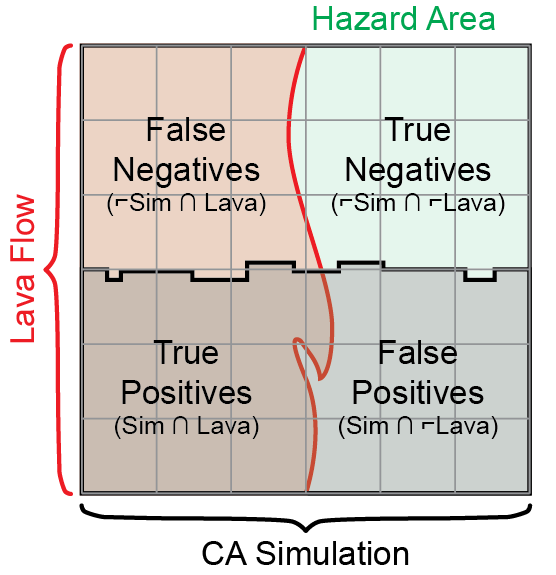
\includegraphics[width=0.4\linewidth]{\FigPath/2xtable_300dpi.png}
			\caption[2x2 table comparing regions inundated by real lava and a simulated flow]{2x2 table comparing regions inundated by real lava and a simulated flow. In the bottom left, True Positives are areas engulfed by lava both in real life and in the simulation. In the top left, False Negatives are areas hit by lava where the simulation failed to model inundation. In the bottom right, False Positives are locations where the simulation forecast inundation, but which remained untouched by lava in reality. Finally, in the top right, True Negatives are areas which were not inundated by lava and the simulation successfully forecast their safety.}
			\label{fig_2x2}
		\end{figure}
		
		Model sensitivity is defined as
		\begin{equation}
			\text{Model~Sensitivity}=\frac{|Lava\cap Sim|}{|Lava|}
		\label{eq_sensitivity}
		\end{equation}
		where $|Lava\cap Sim|$ is the areal size of the interesection of the simulation and the true lava flow (i.e. the True Positives) and $|Lava|$ is the areal size of the lava flow (True Positives and False Negatives). This gives a percentage of the true lava flow that the simulation correctly predicted. 
		
		The Jaccard coefficient, or Jaccard fit, also uses True Positives as the numerator, but expands the denominator to include all areas inundated by either the lava flow or the simulated flow. This is defined as 
		\begin{equation}
			\text{Jaccard~Fit}=\frac{|Lava\cap Sim|}{|Lava\cup Sim|}
		\end{equation}
		where $|Lava\cup Sim|$ is the size of the union of the lava flow and a simulated flow (i.e. True Positives, False Negatives, and False Positives). This gives a percentage of the total area covered by simulated flows and/or true flows that is covered by both.
		
		Each flow algorithm is run using the following parameters (listed in Table \ref{tab_tolbflowparameters}). Flows are run over both 3-arcsecond SRTM topography (75 m grid resolution at 56$^{\circ}$N) and bistatic TanDEM-X topography processed by \citet{kubanek2015lava}. The pulse volume, the volume added to vent cells at each code loop (i.e. each instance of the PULSE module), is set at the product of the grid-cell area (5600 m$^2$ for the SRTM DEM and 225 m$^2$ for the TanDEM-X DEM) and the residual thickness (7.8~m). Both fitness metrics are calculated with the resulting model output, given as a list of inundated locations. ``Failure'' can be defined here as either metric falling below 50\% for the sake of example.
		
		\begin{table}[h]
			\centering
			\caption{Tolbachik Validation Flow Parameters}\\
			\begin{tabular}{l l}
				\toprule
				Elevation Model & 75-m SRTM or 15-m TanDEM-X\\
				Residual Thickness & 7.8~m\\
				Pulse Volumes & 44200 m$^3$ (SRTM) or 1800 m$^3$ (TanDEM-X)\\
				\midrule
				Vent$_N$ Easting & 582800~m (UTM Zone 57)\\
				Vent$_N$ Northing & 6182100~m\\
				Vent$_N$ Total Volume & 4.63$\cdot10^7$~m$^3$\\
				\midrule
				Vent$_S$ Easting & 582475~m\\
				Vent$_S$ Northing & 6180700~m\\
				Vent$_S$ Total Volume & 1.737$\cdot10^8$~m$^3$\\
				\bottomrule
			\end{tabular}
			\label{tab_tolbflowparameters}
		\end{table}
			
	\subsubsection{Results}
	
	\begin{figure}[!h]
			\centering
			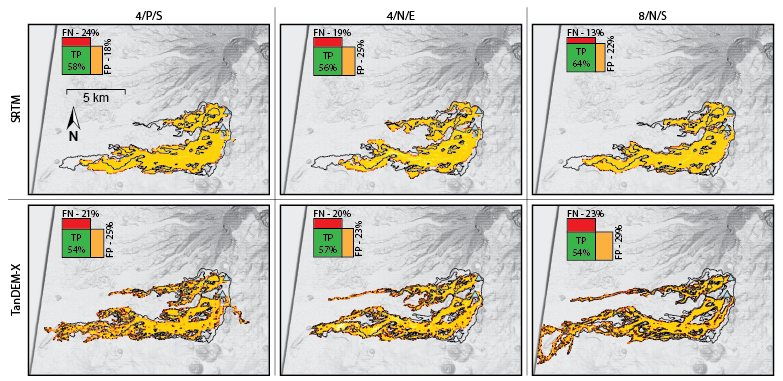
\includegraphics[width=\linewidth]{\FigPath/tolb_lvl3_examples_72dpi}
			\caption[Three simulation algorithms (4/P/S, 4/N/E, and 8/N/S) applied to two elevation models (SRTM and TanDEM-X) to simulate the 2012-3 Tolbachik lava flows, outlined in black]{Three simulation algorithms (4/P/S, 4/N/E, and 8/N/S) applied to two elevation models (SRTM and TanDEM-X) to simulate the 2012-3 Tolbachik lava flows, outlined in black. Lava is emitted from two vent locations marked as blue triangles in the simulation. Diagrams showing the relative True Positives (green), False Positives (orange), and False Negatives (red) are illustrated in the top left of each simulation.}
			\label{fig:tolbachik}
		\end{figure}
	
	
		\begin{table}[h]
		\centering
		\caption{Tolbachik Flow Results}\\
			\begin{tabular}{l c c | c c}
				\toprule
				Transition&\multicolumn{2}{c}{\textbf{SRTM DEM}}&\multicolumn{2}{c}{\textbf{TanDEM-X DEM}}\\
				Function& Jaccard & Sensitivity& Jaccard & Sensitivity\\
				\midrule
				4/P/S & 56.7\%& 76.4\%& 53.0\%& 72.4\% \\
				8/P/S & 61.1  & 80.8  & 46.8  & 67.2   \\
				4/N/S & 57.2  & 77.5  & 44.0  & 64.0   \\
				8/N/S & 63.1  & 82.8  & 46.7  & 67.4   \\
				4/P/E & 51.2  & 71.5  & 54.2  & 73.4   \\
				8/P/E & 58.8  & 78.2  & 56.3  & 76.0   \\
				4/N/E & 54.5  & 74.5  & 55.7  & 73.7   \\
				8/N/E & 59.6  & 78.8  & 56.2  & 75.3   \\
				\bottomrule
			\end{tabular}
			\label{tab_tolbflowresults}
		\end{table}
	
	Three example algorithms are illustrated in Figure \ref{fig:tolbachik}. One primary observation is that all simulations had a longer run-out length on the finer TanDEM-X grid than on the coarser SRTM grid. Despite this, all flows took the correct major pathways taken by the true lava flow. A small diagram in the top left corner of each map in Figure \ref{fig:tolbachik} shows the true positives, false positives, and false negatives in each simulation. True positives are areas inundated by both flow and simulation, false positives are areas simulated as being inundated but are not mapped as such, and false negatives are areas hit by lava that the simulation failed to forecast. 
		
			The best algorithm and DEM pair were the 8/N/S algorithm over SRTM (top left of Figure \ref{fig:tolbachik}), while this same algorithm performed fairly poorly over TanDEM-X topography. For the SRTM simulation, this algorithm achieved a model sensitivity of 82.8\% and a Jaccard fitness score of 63.1\%. Graphically, sensitivity is calculated as the green area in the Figure \ref{fig:tolbachik} diagram divided by the green and red areas. The Jaccard fitness is the green area divided by the total area of the diagram. Because the Jaccard fitness statistic essentially expands the denominator of model sensitivity, it will never be higher than model sensitivity.
			
			If success and failure are defined by having a fits of greater or less than 50\%, all models tested would pass for the SRTM DEM and about half would pass for the TanDEM-X DEM. All but one model (4/P/E) performed worse on the TanDEM-X DEM. The Jaccard fit and Sensitivity for all models are given in Table \ref{tab_tolbflowresults}.
					

